\documentclass[10pt]{beamer}
\mode<beamer>{%
	\usetheme[hideothersubsections,right,width=22mm]{Berkeley}
	%\usetheme{Rochester}
	%\useinnertheme{rounded}
	\usecolortheme{crane}
	%\usecolortheme{rose}
}
\title{Gitflow}
\author[R. Ahangarpour]{Reza Ahangarpour\\[2mm]\tiny{\texttt{ra19@tutanota.com}}}
\institute{Sharif University of Technology}
\titlegraphic{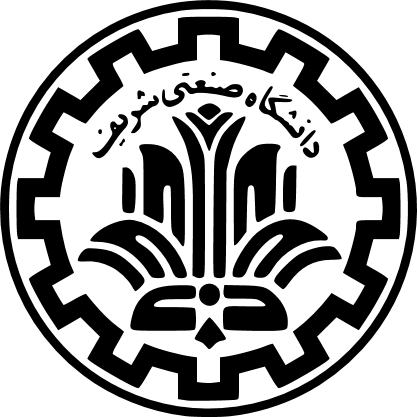
\includegraphics[width=20mm]{sharif.png}}
\date{Jul 22 2022}
\begin{document}
	\begin{frame}
		\titlepage
	\end{frame}
	\begin{frame}
		\frametitle{Outline}
		\tableofcontents[pausesections]
	\end{frame}
	\section{Introduction}
	\begin{frame}
		\frametitle{Git Workflows}
		\begin{definition}
			A \alert{Git workflow} is a recipe or recommendation for how to use Git.
		\end{definition}
		\pause
		\begin{example}
			\begin{itemize}
				\item[$\lozenge$] Centralized workflow \pause
				\item[$\lozenge$] Feature branch workflow \pause
				\item[$\lozenge$] \alert{Gitflow} workflow \pause
				\item[$\lozenge$] Forking workflow
			\end{itemize}
		\end{example}
	\end{frame}
	\section{Branches}
	\subsection{Overview}
	\begin{frame}
		\frametitle{Gitflow Branches}
		\begin{block}{Branches}
			\begin{itemize}
				\item[$\lozenge$] Main
				\item[$\lozenge$] Develop
				\item[$\lozenge$] Features
				\item[$\lozenge$] Release
				\item[$\lozenge$] Hotfix
			\end{itemize}
		\end{block}
	\end{frame}
	\subsection{Main and Develop}
	\begin{frame}
		\frametitle{Gitflow Branches}
		\framesubtitle{Main and Develop Branches}
		ghfh
	\end{frame}
	\begin{frame}
		\frametitle{What's Still To Do?}
		\begin{columns}[t]
			\column{.5\textwidth}
			\begin{block}{Answered Question}
				How many primes are there?
			\end{block}
			\column{.5\textwidth}
			\begin{block}{Open Question}
				Is every even number the sum of two primes?
			\end{block}
		\end{columns}
	\end{frame}
	\subsection{Results}
	\begin{frame}
		\frametitle{There Is No Largest Prime Number}
		\framesubtitle{The proof uses \texttt{reductio ad absurdum}.}
		\begin{theorem}
			There is no largest prime number.
		\end{theorem}
		\only<4->{The proof used \texttt{reductio ad absurdum}.}
		\begin{proof}
			\begin{enumerate}
				\item<1-| alert@1> Suppose $p$ where the largest prime.
				\item<2-> Let $\sigma$ be the product of the first $p$ numbers.
				\item<3-> Then $\sigma+1$ is not divisible by any of them.
				\item<1-> But $\sigma+1$ is greater than $1$, thus divisible by some prime
					number not in the first $\sigma$ number.\qedhere
			\end{enumerate}
		\end{proof}
	\end{frame}
	\begin{frame}[fragile]
		\frametitle{Sieve of Eratosthenes}
		\framesubtitle{\texttt{+\#Prime Factors}}
		\begin{block}{C Code}
		\begin{verbatim}[xleftmargin=7mm]
#define N 10000000
int i=2,j,a[N];
int main(){
	for(;i<N;i++)if(!a[i])
		for(j=i;j<N;j+=i)a[j]++;
	return 0;
}
		\end{verbatim}
		\end{block}
		\visible<2>{Note the use of \texttt{a[j]++}.}
	\end{frame}
	\begin{frame}
	\end{frame}
\end{document}
